\documentclass{beamer}
\usepackage{amsmath,amsfonts}	% use math symbols
\usepackage{graphicx} % insert images
\usepackage{url} % insert urls
\usepackage{subfigure}

\usepackage{amssymb}
\usepackage{amsmath}
\usepackage{bm}

\usepackage{algpseudocode}
\usepackage{algorithm}

\usepackage{multirow}
\usepackage{rotating}



%%%%%%%%%%%%%%%%%%%%%%%%%%%%%%%%%%%%%%%%%%%%%%%%%%%%%%%%%%%%%%%%%%%%%%%%%%%%%%%%




\def\Tiny{\fontsize{5pt}{5pt}\selectfont}


% Setup TikZ

\usepackage{tikz}
\usetikzlibrary{arrows}
%\usetikzlibrary{mindmap,trees}
\tikzstyle{block}=[draw opacity=0.7,line width=1.4cm]


\mode<presentation>
{
\usetheme{Warsaw}

%\usetheme{Antibes}	% tree outline, neat
%\usetheme{JuanLesPins}	% like Antibes, with shading
%\usetheme{Bergen}	% outline on side
%\usetheme{Luebeck}	% like Warsaw, square sides
%\usetheme{Berkeley}	% interesting left bar outline
%\usetheme{Madrid}	% clean, nice.  7/12 page numbers
%\usetheme{Berlin}	% dots show slide number
%\usetheme{Malmoe}	% OK, plain, unshaded
%\usetheme{Boadilla}	% nice, white bg, no top bar
%\usetheme{Marburg}	% nice, outline on right
%\usetheme{boxes}	% ???
%\usetheme{Montpellier}	% tree outline on top, plainish white
%\usetheme{Copenhagen}	% like Warsaw
%\usetheme{PaloAlto}	% looks good
%\usetheme{Darmstadt}	% like Warsaw with circle outline
%\usetheme{Pittsburgh}
%\usetheme{default}
%\usetheme{Rochester}	% like boxy, unshaded warsaw
%\usetheme{Dresden}	% circle outline on top
%\usetheme{Singapore}	% purple gradient top
%\usetheme{Frankfurt}	% like Warsaw with circle outline on top
%\usetheme{Szeged}
%\usetheme{Goettingen}	% light purple right bar outline
%\usetheme{Warsaw}
%\usetheme{Hannover}	% like Goett with bar on left
%\usetheme{compatibility}
%\usetheme{Ilmenau}

%\usefonttheme{serif}

  \setbeamercovered{transparent}
  % or whatever (possibly just delete it)
}


\usepackage[english]{babel}
% or whatever

%\usepackage[latin1]{inputenc}
% or whatever

\usepackage{times}
%\usepackage[T1]{fontenc}
% Or whatever. Note that the encoding and the font should match. If T1
% does not look nice, try deleting the line with the fontenc.


\title[Intruction to Data Mining] % (optional, use only with long paper titles)
{Introduction to Data Mining}

%\subtitle
%{Include Only If Paper Has a Subtitle}

\subtitle
{Small and Big Data}

%\author[Author, Another] % (optional, use only with lots of authors)
%{F.~Author\inst{1} \and S.~Another\inst{2}}
%% - Give the names in the same order as the appear in the paper.
%% - Use the \inst{?} command only if the authors have different
%%   affiliation.



\author[]
{
  Daniel Rodriguez %\inst{1} \and
  \and David F. Barrero
%   R Ruiz\inst{2} \and
%   J C Riquelme\inst{3} \and
%   R Harrison\inst{4}
  %\textcolor{green!50!black}{Daniel Rodriguez}\inst{1}
}


%\institute[Universities of Somewhere and Elsewhere] % (optional, but mostly needed)
%{
%  \inst{1}%
%  Department of Computer Science\\
%  University of Somewhere
%  \and
%  \inst{2}%
%  Department of Theoretical Philosophy\\
%  University of Elsewhere}
%% - Use the \inst command only if there are several affiliations.
%% - Keep it simple, no one is interested in your street address.

\institute[Univ of Alcala]
{
  %\inst{1}%
  University of Alcala, Spain
%   \and
%   \vskip-2mm
%   \inst{2}%
%   Pablo de Olavide University, Seville
%  \and
%   \vskip-2mm
%   \inst{3}%
%    University of Seville, Seville
%  \and
%   \vskip-2mm
%   \inst{3}%
%    Oxford Brookes University, UK
}


\date[] % (optional, should be abbreviation of conference name)
{AI Session}
% - Either use conference name or its abbreviation.
% - Not really informative to the audience, more for people (including
%   yourself) who are reading the slides online

\subject{Introduction to Data Mining}
% This is only inserted into the PDF information catalog. Can be left
% out.


% If you have a file called "university-logo-filename.xxx", where xxx
% is a graphic format that can be processed by latex or pdflatex,
% resp., then you can add a logo as follows:

\pgfdeclareimage[height=0.5cm]{university-logo}{logoUAH}
\logo{\pgfuseimage{university-logo}}


% Delete this, if you do not want the table of contents to pop up at
% the beginning of each subsection:
\AtBeginSubsection[]
{
  \begin{frame}<beamer>{Outline}
    \tableofcontents[currentsection,currentsubsection]
  \end{frame}
}

% If you wish to uncover everything in a step-wise fashion, uncomment
% the following command:

%\beamerdefaultoverlayspecification{<+->}


%%%%%%%%%%%%%%%%%%%%%%%%%%%%%%%%%%%%%%%%%%%%%%%%%%%%%%%%%%%%%%%%%%%%%%%%%%%%%%%%

\begin{document}

\maketitle


%%%%%%%%%%%%%%%%%%%%%%%%%%%%%%%%%%%%%%%%%%%%%%%%%%%%%%%%%%%%%%%%%%%%%%%%%%%%%%%%
%%%%%%%%%%%%%%%%%%%%%%%%%%%%%%%%%%%%%%%%%%%%%%%%%%%%%%%%%%%%%%%%%% Introduction
\section{Introduction}

%%%%%%%%%%%%%%%%%%%%%%%%%%%%%%%%%%%%%%%%%%%%%%%%%%%%%%%%%%%%%%%%%%%%%%%%%%%%%%%
\subsection{What is Knowledge Discovery in Databases?}

%%%%%%%%%%%%%%%%%%%%%%%%%%%%%%%%%%%%%%%%%%%%%%%%%%%%%%%%%%%%%%%%%%%%%%%%%%%%%%%
\begin{frame}{What is Data Mining?}



\begin{block}{Data Mining}
\begin{itemize}
 \item It is process of discovering \textit{structural patterns} in data \cite{WFH11}. %[Witten and Frank, 2005].
    \begin{itemize}
      \item The \alert{patterns} discovered must be meaningful in that they lead to some advantage
      \item \emph{Structural} Patterns mined are represented in terms of a structure that can be
examined, reasoned about, and used to inform future decisions (help to explain something about the data)
      
    \end{itemize}
    \item The process must be (semi)automatic
    \item It can be used to classify/predict unknown examples
    \item We will need more and more \alert{data scientist}!
\end{itemize}
\end{block}


\end{frame}

%%%%%%%%%%%%%%%%%%%%%%%%%%%%%%%%%%%%%%%%%%%%%%%%%%%%%%%%%%%%%%%%%%%%%%%%%%%%%%%%
\begin{frame}{Data Mining}

%The process of discovering structural patterns in data \cite{WFH11}.
%[Witten and Frank, 2005]

\begin{block}{Data...}
\begin{itemize}
 \item \alert{Data} is increasing without an end. The amount of data stored doubles every 20 months.
    \begin{itemize}
      \item The Web overwhelms us with information
      \item Electronic devices (smartphones), supermarkets, financial habits, health... 
    \end{itemize}
\end{itemize}
\end{block}
\vspace{-2mm}
\begin{block}{... Mining}
\begin{itemize}
 \item Looking for patterns in data.
    \begin{itemize}
      \item It like extracting large volume of earth \& raw material (data) from a mine, process
it, obtain a small amount of very precious material (model with valuable use)
      \item Analyzing data intelligently can lead to new insights and, in commercial settings, to competitive advantages
    \end{itemize}
\end{itemize}
\end{block}

\end{frame}



%%%%%%%%%%%%%%%%%%%%%%%%%%%%%%%%%%%%%%%%%%%%%%%%%%%%%%%%%%%%%%%%%%%%%%%%%%%%%%%%
% \begin{frame}{What is Data Mining?}
% 
% \begin{tikzpicture}[scale=0.9]
%   \path[mindmap,concept color=black,text=white]
%     node[concept] {Computer Science}
%     [clockwise from=0]
%     child[concept color=green!50!black] {
%       node[concept] {practical}
%       [clockwise from=90]
%       child { node[concept] {algorithms} }
%       child { node[concept] {data structures} }
%       child { node[concept] {pro\-gramming languages} }
%       child { node[concept] {software engineer\-ing} }
%     }  
%     child[concept color=blue] {
%       node[concept] {applied}
%       [clockwise from=-30]
%       child { node[concept] {databases} }
%       child { node[concept] {WWW} }
%     }
%     child[concept color=red] { node[concept] {technical} }
%     child[concept color=orange] { node[concept] {theoretical} };
% \end{tikzpicture}
% 
% \end{frame}

%%%%%%%%%%%%%%%%%%%%%%%%%%%%%%%%%%%%%%%%%%%%%%%%%%%%%%%%%%%%%%%%%%%%%%%%%%%%%%%%
\begin{frame}{What is Data Mining?}

%\begin{tikzpicture}
%   \tikzset{venn circle/.style={draw,circle,minimum width=6cm,fill=#1,opacity=0.4}}
% 
%   \node [venn circle = red] (A) at (0,0) {$A$};
%   \node [venn circle = blue] (B) at (60:4cm) {$B$};
%   \node [venn circle = green] (C) at (0:4cm) {$C$};
%   \node[left] at (barycentric cs:A=1/2,B=1/2 ) {$A \cap B$}; 
%   \node[below] at (barycentric cs:A=1/2,C=1/2 ) {$A \cap C$};   
%   \node[right] at (barycentric cs:B=1/2,C=1/2 ) {$B \cap C$};   
%   \node[below] at (barycentric cs:A=1/3,B=1/3,C=1/3 ){$A \cap B \cap C$};
% \end{tikzpicture} 

\begin{center}
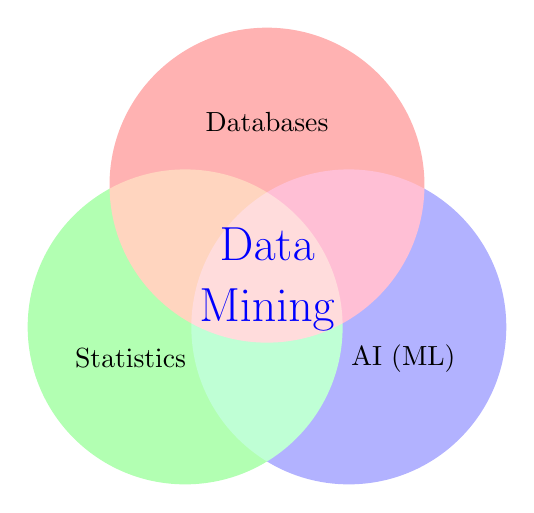
\begin{tikzpicture}
  \begin{scope}[blend group=soft light]
    \fill[red!30!white] ( 90:1.2) circle (2); 
    \fill[green!30!white] (210:1.2) circle (2); 
    \fill[blue!30!white] (330:1.2) circle (2);
  \end{scope}
  \node at ( 90:2) {Databases};
  \node at (210:2) {Statistics}; 
  \node at (330:2) {AI (ML)}; 
  %\node [font=\Large] {Data Mining};
  \node [font=\LARGE, align=center, color=blue] {Data \\Mining};
\end{tikzpicture}
 \end{center}

\end{frame}

%%%%%%%%%%%%%%%%%%%%%%%%%%%%%%%%%%%%%%%%%%%%%%%%%%%%%%%%%%%%%%%%%%%%%%%%%%%%%%%%
\begin{frame}{Confusing terms}

\begin{itemize}
    \item \alert{Data Mining} = Statistics + Databases + Artificial Intelligence
    \item \alert{Machine Learning} = Field of AI
    \item \alert{Statistics} = Field of Mathematics
    \item \alert{Big data} = A lot of data
    \item \alert{ML engineer} = Professional role
    \item \alert{Data scientist} = Professional role
    \item \alert{KDD} = A process
\end{itemize}

\end{frame}



%%%%%%%%%%%%%%%%%%%%%%%%%%%%%%%%%%%%%%%%%%%%%%%%%%%%%%%%%%%%%%%%%%%%%%%%%%%%%%%%
\subsection{Knowledge Discovery in Databases}

%%%%%%%%%%%%%%%%%%%%%%%%%%%%%%%%%%%%%%%%%%%%%%%%%%%%%%%%%%%%%%%%%%%%%%%%%%%%%%%%
\begin{frame}{What is Knowledge Discovery in Databases?}

% \begin{itemize}
%   \item KDD is the automatic extraction of non-obvious, hidden knowledge from large volumes of data
% \end{itemize}

\begin{block}{}
The non-trivial process of identifying valid, novel, potentially useful, and ultimately understandable patterns in data - Fayyad, Piatetsky-Shapiro, Smyth (1996)
\end{block}

\begin{center}
\begin{tabular}{l|l}
non-trivial process &  multiple processes\\
valid & justified patterns/models\\
novel & previously unknown\\
useful &  can be used\\
understandable & by human and/or machine
\end{tabular}
\end{center}


\end{frame}

%%%%%%%%%%%%%%%%%%%%%%%%%%%%%%%%%%%%%%%%%%%%%%%%%%%%%%%%%%%%%%%%%%%%%%%%%%%%%%%%
\subsection{Applications}

%%%%%%%%%%%%%%%%%%%%%%%%%%%%%%%%%%%%%%%%%%%%%%%%%%%%%%%%%%%%%%%%%%%%%%%%%%%%%%%%
\begin{frame}{Applications}

It is just a (fantastic) tool that can be applied everywhere!
\begin{itemize}
    \item If there are data, you can use DM
    \item If there are no data, you can gather it and use DM
\end{itemize}

Business information

\begin{itemize}
 \item Marketing and sales data analysis
 \item Investment analysis
 \item Loan approval
 \item Fraud detection
 \item etc
\end{itemize}

\end{frame}


%%%%%%%%%%%%%%%%%%%%%%%%%%%%%%%%%%%%%%%%%%%%%%%%%%%%%%%%%%%%%%%%%%%%%%%%%%%%%%%%
\begin{frame}{Recommender Systems}

Recommender systems

\begin{center}
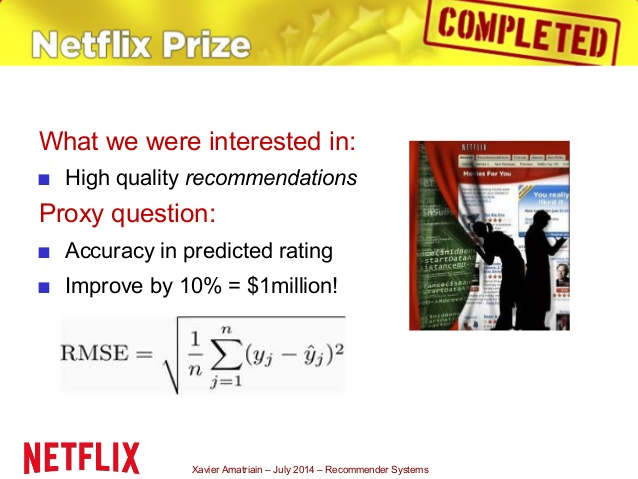
\includegraphics[width=.7\textwidth]{figs/recommender-systems}
\end{center}

\end{frame}

%%%%%%%%%%%%%%%%%%%%%%%%%%%%%%%%%%%%%%%%%%%%%%%%%%%%%%%%%%%%%%%%%%%%%%%%%%%%%%%%
\begin{frame}{Social Networks}

\begin{center}
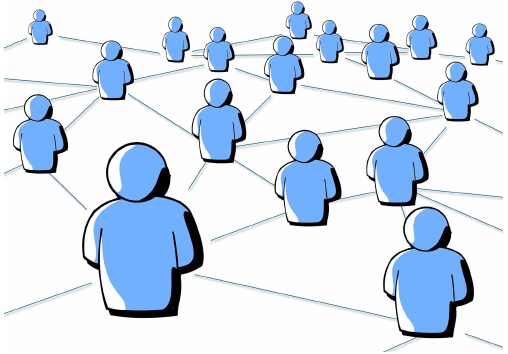
\includegraphics[width=.8\textwidth]{figs/SocialNetworks}
\end{center}

\end{frame}

%%%%%%%%%%%%%%%%%%%%%%%%%%%%%%%%%%%%%%%%%%%%%%%%%%%%%%%%%%%%%%%%%%%%%%%%%%%%%%%%
\begin{frame}{Games}

\begin{center}

\includegraphics[width=.45\textwidth,keepaspectratio=true]{figs/games}
\end{center}

\end{frame}

%%%%%%%%%%%%%%%%%%%%%%%%%%%%%%%%%%%%%%%%%%%%%%%%%%%%%%%%%%%%%%%%%%%%%%%%%%%%%%%%
\begin{frame}{Robotics, Autonomous cars, etc}


\begin{center}
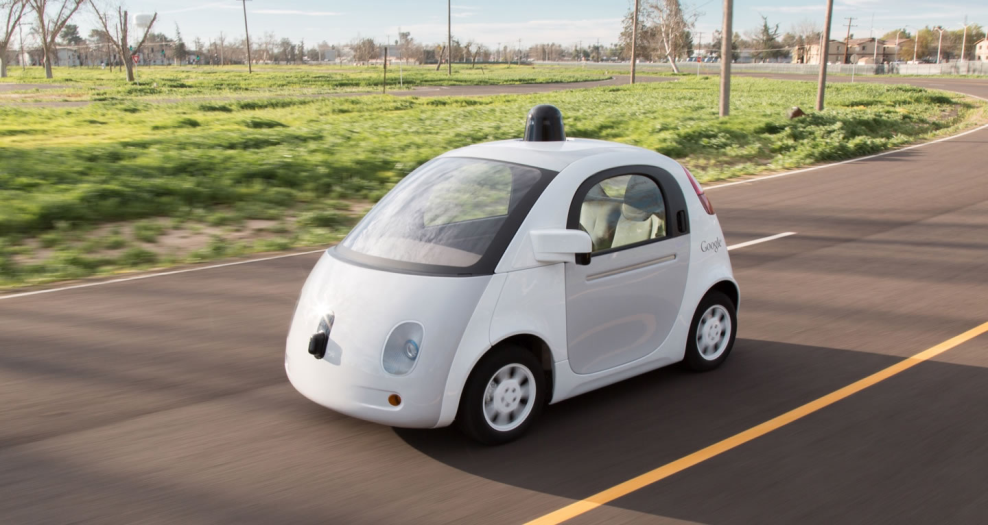
\includegraphics[width=.9\textwidth,,keepaspectratio=true]{figs/autonomousCar}
\end{center}

\end{frame}

%%%%%%%%%%%%%%%%%%%%%%%%%%%%%%%%%%%%%%%%%%%%%%%%%%%%%%%%%%%%%%%%%%%%%%%%%%%%%%%%
\begin{frame}{Computer Vision}

Computer vision
  
\begin{center}
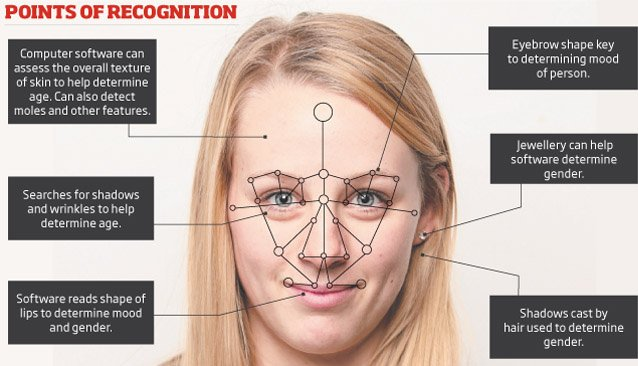
\includegraphics[width=.9\textwidth]{figs/FaceRecognition}
\end{center}

\end{frame}

%%%%%%%%%%%%%%%%%%%%%%%%%%%%%%%%%%%%%%%%%%%%%%%%%%%%%%%%%%%%%%%%%%%%%%%%%%%%%%%%
\begin{frame}{Scientific information}

\begin{itemize}
 \item Sky survey cataloging
 \item Biosequence Databases
 \item Geosciences: Quakefinder
 \item etc.
\end{itemize}

\begin{center}
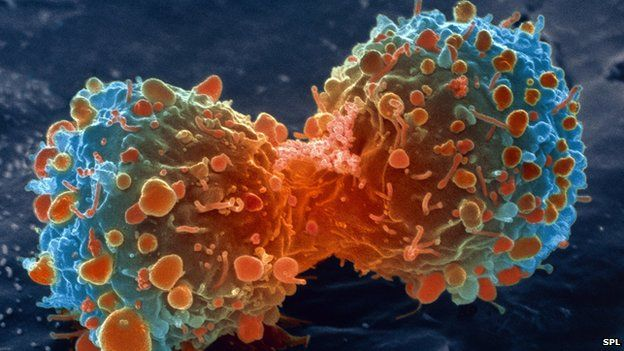
\includegraphics[width=.3\textwidth]{figs/bioinformatics}
\end{center}

\end{frame}

%%%%%%%%%%%%%%%%%%%%%%%%%%%%%%%%%%%%%%%%%%%%%%%%%%%%%%%%%%%%%%%%%%%%%%%%%%%%%%%%
\begin{frame}{Application examples}

Robotics
\begin{itemize}
    \item MarI/O - Machine Learning for Video Games \href{https://www.youtube.com/watch?v=qv6UVOQ0F44}{(Video)}
    \item Artificial vision \href{https://www.youtube.com/watch?v=4KlYdCBdjEg}{(Video)}
    \item Machine Learning \href{https://www.youtube.com/watch?v=pgaEE27nsQw}{(Video)}
    \item Reinforcement Learning \href{https://www.youtube.com/watch?v=W\_gxLKSsSIE}{(Video)}
    \item Evolved Electrophysiological Soft Robots \href{https://www.youtube.com/watch?v=HgWQ-gPIvt4}{(Video)}
\end{itemize}

Deep learning
\begin{itemize}
    \item DeepBach \href{https://www.youtube.com/watch?v=QiBM7-5hA6o}{(Video)}
    \item Deep Neural Network learns Van Gogh's \href{https://www.youtube.com/watch?v=-R9bJGNHltQ}{(Video)}
    \item Deep Learning on Drones \href{https://www.youtube.com/watch?v=wSFYOw4VIYY}{(Video)}
    \item Emotion recognition \href{https://www.youtube.com/watch?v=PL3xJErjEgU}{(Video)}
\end{itemize}


\end{frame}


%%%%%%%%%%%%%%%%%%%%%%%%%%%%%%%%%%%%%%%%%%%%%%%%%%%%%%%%%%%%%%%%%%%%
%%%%%%%%%%%%%%%%%%%%%%%%%%%%%%%%%%%%%%%%%%%%%%%%%%%%%%%%%%%%%%%%%%%% 

\section{Data Mining/KDD Process}
%%%%%%%%%%%%%%%%%%%%%%%%%%%%%%%%%%%%%%%%%%%%%%%%%%%%%%%%%%%%%%%%%%%% 

\begin{frame}{Data Mining/KDD Process}

\begin{itemize}
 \item Data integration, Selection, cleaning and transformation of data
 \item Machine Learning (patterns)., classifiers, rules, etc
 \item Evaluation and interpretation
 \item Decision making (knowledge)
\end{itemize}

\begin{center}
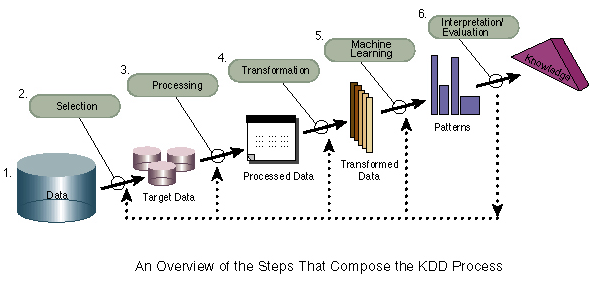
\includegraphics[width=.8\textwidth]{figs/DMProcess}
\end{center}

\end{frame}

%%%%%%%%%%%%%%%%%%%%%%%%%%%%%%%%%%%%%%%%%%%%%%%%%%%%%%%%%%%%%%%%%%%%
\subsection{KDD Process: Integration}

%%%%%%%%%%%%%%%%%%%%%%%%%%%%%%%%%%%%%%%%%%%%%%%%%%%%%%%%%%%%%%%%%%%%
\begin{frame}{KDD Process: Integration}

\begin{center}
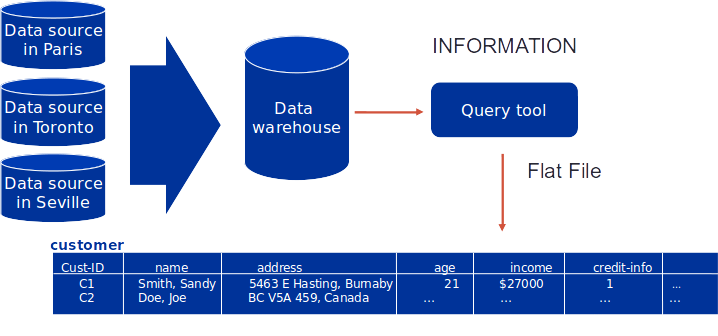
\includegraphics[width=.8\textwidth]{figs/DataIntegration}
\end{center}

Instances characterized by the values of features (attributes) that measure
different aspects of the instance.

\end{frame}

%%%%%%%%%%%%%%%%%%%%%%%%%%%%%%%%%%%%%%%%%%%%%%%%%%%%%%%%%%%%%%%%%%%%
\subsection{KDD Process: Selection, cleaning and transformation}

%%%%%%%%%%%%%%%%%%%%%%%%%%%%%%%%%%%%%%%%%%%%%%%%%%%%%%%%%%%%%%%%%%%%
\begin{frame}{KDD Process: Selection, cleaning and transformation}

\begin{itemize}
 \item Removing outliers
 \item Data sampling (if we have too much data we can select instances)
 \item Missing values
 \item Noisy data: wrongly recorded values
 \item Feature selection: removing redundant and irrelevant attributes
 \item Derive new attributes from existing ones, e.g., population density from from inhabitant and area
 \item Data transformation: discretization, normalization
\end{itemize}


\end{frame}


%%%%%%%%%%%%%%%%%%%%%%%%%%%%%%%%%%%%%%%%%%%%%%%%%%%%%%%%%%%%%%%%%%%%
\subsection{Machine learning}

%%%%%%%%%%%%%%%%%%%%%%%%%%%%%%%%%%%%%%%%%%%%%%%%%%%%%%%%%%%%%%%%%%%%
\begin{frame}{KDD Model Classification}

\begin{itemize}
 \item DM algorithms are traditionally divided into:
 \item \alert{Supervised learning} which aims to discover knowledge for classification or prediction (\emph{predictive})
 \item \alert{Unsupervised learning} which refers to the induction to extract interesting knowledge from data (\emph{descriptive}).

\end{itemize}

There are also semi-supervised approaches: goal is classification but the input contains both unlabeled and labeled data.

Subgroup Discovery approaches generate descriptive rules are also half way between descriptive and predictive techniques.

\end{frame}


%%%%%%%%%%%%%%%%%%%%%%%%%%%%%%%%%%%%%%%%%%%%%%%%%%%%%%%%%%%%%%%%%%%%
\begin{frame}{Supervised Learning}


\begin{itemize}
  \item A classifier resembles a function in the sense that it attaches a value (or a range or a description) to a set of attribute values. It induces a classification model.

  \item Given $m$ instances (samples) characterized by $n$ predicted attributes, $A_1, \ldots, A_n$, and the class variable, $C$

%     \begin{itemize}
%       \item Numeric class (regression) or discrete (classification)
%     \end{itemize}
\end{itemize}
      
\begin{center}
\begin{tabular}{l|lll|l}
  & $X_1 $ & $\ldots$ & $X_n$ & $C_M$ \\
  \hline
$(\mathbf{x}^{(1)}, C^{(1)})$ & $x^{(1)}_1$ & $\ldots$ & $x^{(1)}_n$ & $C^{(1)}_M$ \\
$(\mathbf{x}^{(2)}, C^{(2)})$ & $x^{(2)}_1$ & $\ldots$ & $x^{(2)}_n$ & $C^{(2)}_M$ \\
\ldots\ldots 	 &		& \ldots 	&		& \ldots \\	
  \hline
$(\mathbf{x}^{(N)}, C^{(N)})$ & $x^{(N)}_1$ & $\ldots$ & $x^{(N)}_n$ & $C^{(N)}_M$ \\
\hline
$(\mathbf{x}^{(N+1)}, C^{(N+1)})$ & $x^{(N+1)}_1$ & $\ldots$ & $x^{(N+1)}_n$ & $??$ \\
\end{tabular}
\end{center}


\end{frame}

%%%%%%%%%%%%%%%%%%%%%%%%%%%%%%%%%%%%%%%%%%%%%%%%%%%%%%%%%%%%%%%%%%%%%%%%%%%%%%%%
\begin{frame}{Supervised Learning}

\begin{center}
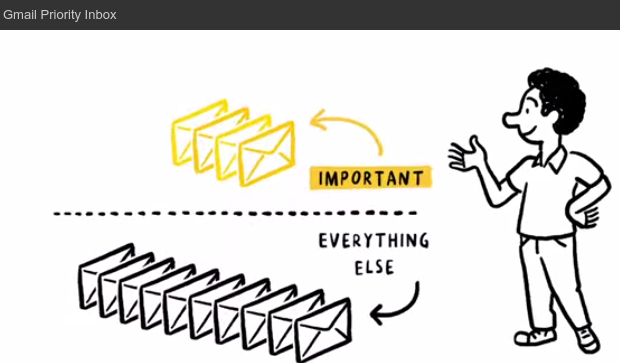
\includegraphics[width=.9\textwidth]{figs/selectionGmail}
\end{center}

\end{frame}


%%%%%%%%%%%%%%%%%%%%%%%%%%%%%%%%%%%%%%%%%%%%%%%%%%%%%%%%%%%%%%%%%%%%%%%%%%%%%%%%
\begin{frame}{Supervised Learning: Models}

\begin{itemize}
\item \alert{Decision trees} Trees where each leaf indicates a class and internal nodes specifies some test to be carried out (e.g. C4.5). 

\item \alert{Rule induction}
  \begin{itemize}
  \item \texttt{\textbf{If} condition \textbf{then} class} 
  \item \texttt{\textbf{If} ... \texttt{then} ... \textbf{else if} ...} (hierarchical rules)
  \end{itemize}

\item \alert{Lazy techniques} store previous instances and search similar ones when performing classification with new instances
  \begin{itemize}
  \item $k$-\emph{Nearest Neighbour} ($k$-NN) is a method for classifying objects based on closest training example(s) in the feature space.
  \end{itemize}
       
\end{itemize}

\end{frame}

%%%%%%%%%%%%%%%%%%%%%%%%%%%%%%%%%%%%%%%%%%%%%%%%%%%%%%%%%%%%%%%%%%%%%%%%%%%%%%%%
\begin{frame}{Supervised Learning: Models (Cont.)}

\begin{itemize}
\item \alert{Regression} techniques (numerical prediction)
\item \alert{Neural Networks} are composed by a set of nodes (units, neurons, processing elements) where each node has input and output and performs a simple computation by its node function.

\item \alert{Statistical techniques}. For example:
    \begin{itemize}
    \item Bayesian networks classifiers assign a set of attributes $A_1, A_2,..., A_n$ to a class $C_j$ such that $P(C_j | A_1, A_2,\ldots, A_n)$ is maximal
    \end{itemize}

\item \alert{Meta-techniques} combine \emph{multiple classifier models} (there are several ways to do so)          
\end{itemize}

\end{frame}


%%%%%%%%%%%%%%%%%%%%%%%%%%%%%%%%%%%%%%%%%%%%%%%%%%%%%%%%%%%%%%%%%%%%%%%%%%%%%%%%
\begin{frame}{Supervised Learning: Numeric Prediction}

\begin{center}
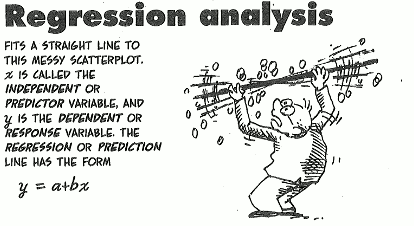
\includegraphics[width=.9\textwidth]{figs/regressionCarton}
\end{center}

\end{frame}

%%%%%%%%%%%%%%%%%%%%%%%%%%%%%%%%%%%%%%%%%%%%%%%%%%%%%%%%%%%%%%%%%%%%%%%%%%%%%%%%
\begin{frame}{Unsupervised Learning}

There is no ‘class’ attribute

\begin{itemize}
 \item \alert{Clustering}
 \begin{itemize}
  \item Tree clustering: join together objects (e.g., animals) into successively larger clusters, using some measure of similarity or distance.
  \item Algorithms: K-Means, EM (Expectation Maximization)
 \end{itemize}

 \item \alert{Association rules}, e.g., rules among supermarket items
 \begin{itemize}
  \item Algorithms: APRIORI, etc.
 \end{itemize}

\end{itemize}


\begin{center}
\begin{tabular}{l|lll}
  & $X_1 $ & $\ldots$ & $X_n$  \\
  \hline
$(\mathbf{x}^{(1)}, C^{(1)})$ & $x^{(1)}_1$ & $\ldots$ & $x^{(1)}_n$ \\
$(\mathbf{x}^{(2)}, C^{(2)})$ & $x^{(2)}_1$ & $\ldots$ & $x^{(2)}_n$ \\
\ldots\ldots 	 &		& \ldots  &	\\	
$(\mathbf{x}^{(N)}, C^{(N)})$ & $x^{(N)}_1$ & $\ldots$ & $x^{(N)}_n$ \\
\end{tabular}
\end{center}

\end{frame}

%%%%%%%%%%%%%%%%%%%%%%%%%%%%%%%%%%%%%%%%%%%%%%%%%%%%%%%%%%%%%%%%%%%%%%%%%%%%%%%%
\begin{frame}{Unupervised Learning: Clustering}

\begin{center}
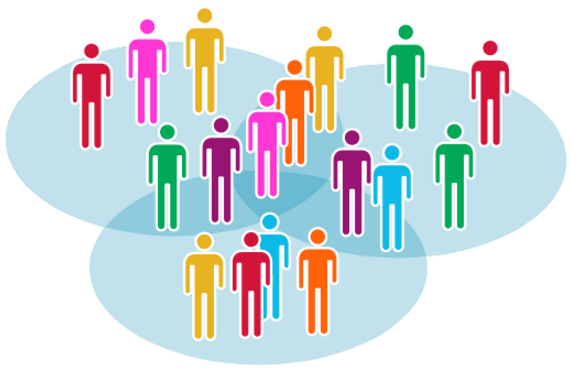
\includegraphics[width=.7\textwidth]{figs/clustering}
\end{center}

\end{frame}

%%%%%%%%%%%%%%%%%%%%%%%%%%%%%%%%%%%%%%%%%%%%%%%%%%%%%%%%%%%%%%%%%%%%%%%%%%%%%%%%
\begin{frame}{Unupervised Learning: Association Rules}

\begin{center}
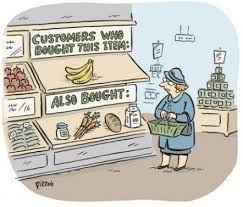
\includegraphics[width=.7\textwidth]{figs/associationRules}
\end{center}

\end{frame}


%%%%%%%%%%%%%%%%%%%%%%%%%%%%%%%%%%%%%%%%%%%%%%%%%%%%%%%%%%%%%%%%%%%%%%%%%%%%%%%%
% \subsection{Model examples}
% 

%%%%%%%%%%%%%%%%%%%%%%%%%%%%%%%%%%%%%%%%%%%%%%%%%%%%%%%%%%%%%%%%%%%%
%%%%%%%%%%%%%%%%%%%%%%%%%%%%%%%%%%%%%%%%%%%%%%%%%%%%% Evaluation 
\section{Evaluation}

%%%%%%%%%%%%%%%%%%%%%%%%%%%%%%%%%%%%%%%%%%%%%%%%%%%%%%%%%%%%%%%%%%%%

\subsection{Evaluation of Supervised Models}

%%%%%%%%%%%%%%%%%%%%%%%%%%%%%%%%%%%%%%%%%%%%%%%%%%%%%%%%%%%%%%%%%%%%
\begin{frame}{Evaluation of Supervised Models}

\begin{itemize}
 \item Once we obtain the supervised model with the training data, we need to evaluate it with some new data (testing data)
 
 \begin{itemize}
  \item We cannnot use the the same data for training and testing. E.g. evaluating a student with exercises previouly solved. Student ‘s marks will be optimistic and we don’t know about student capability to generalise learned concepts.
 \end{itemize}

\end{itemize}


\end{frame}


%%%%%%%%%%%%%%%%%%%%%%%%%%%%%%%%%%%%%%%%%%%%%%%%%%%%%%%%%%%%%%%%%%%%
\begin{frame}{Holdout approach}


\alert{Holdout approach} consists of dividing the dataset into training (approx. 2/3 of the data) and testing (approx 1/3 of the data).

Problems: Skewed data, missing classes, etc. if randomly divided

\alert{Stratification} ensures that each class is represented with approximately equal proportions, e.g., if data contains aprox 45\% of positive cases, the training and testing datasets should mantain similar proportion of positive cases. 

Holdout estimate can be made more reliable by repeating the process with different subsamples (\alert{repeated holdout method})

The error rates on the different iterations are averagerate)
\end{frame}


%%%%%%%%%%%%%%%%%%%%%%%%%%%%%%%%%%%%%%%%%%%%%%%%%%%%%%%%%%%%%%%%%%%%
\begin{frame}[shrink]{Cross Validation}

\begin{columns}
 
\column{0.8\textwidth}
\alert{Cross-validation} (CV) avoids overlapping test sets. The $k$-fold CV consists on:
\begin{itemize}
 \item First step: split dataset ($\mathcal{D}$) into $k$ subsets of equal size $C_1,\ldots,C_k$. Subsets are generally stratified before the CV is performed

 \item Second step: we construct a dataset $D_i = D-C_i$ used for \emph{training} and test the accuracy of the classifier $f(D_i)$ on $C_i$ subset for \textit{testing}
 
\end{itemize}

The error estimates are averaged to yield an overall error estimate, i.e., having done this for all $k$, usually $k=10$, we estimate the accuracy of the method by averaging the accuracy over the $k$ cross-validation.

\column{0.2\textwidth}
\begin{center}
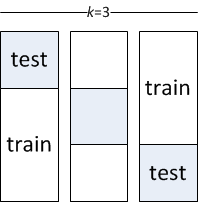
\includegraphics[width=\textwidth]{figs/crossValidation}
\end{center}

\end{columns}

\end{frame}

%%%%%%%%%%%%%%%%%%%%%%%%%%%%%%%%%%%%%%%%%%%%%%%%%%%%%%%%%%%%%%%%%%%%
\begin{frame}{Confusion matrix}

\alert{Confusion matrix} 

% \begin{table}
% \centering
% \scriptsize
%  \caption{Confusion Matrix for Two Classes}
%  \label{tab:confMatrix}
\begin{tabular}{cc||p{2.5cm}|p{2.5cm}||p{2.5cm}}
  & & \multicolumn{2}{c}{\emph{Actual}}\\
  & &    \emph{Pos} & \emph{Neg} \\
  \hline\hline
  \multirow{6}{*}{\emph{Pred}}
  &\emph{Pos} & True Pos \newline ($TP$)  &  False Pos \newline ($FP$)  \newline (False alarm) & $PPV=$\newline $Conf= \newline Prec=\frac{TP}{TP+FP}$ \\
  %\hline
  \cline{2-5}
  &\emph{Neg} & False Neg \newline  ($FN$)   &  True Neg\newline ($TN$) & $NPV=\frac{TN}{FN+TN}$\\
  \hline
  &  & $Recall=\newline Sens=\newline TP_r= \frac{TP}{TP+FN}$ & $Spec= \newline TN_r= \frac{TN}{FP+TN} $ & \\
  %\hline
\end{tabular}
% \end{table}

\end{frame}

%%%%%%%%%%%%%%%%%%%%%%%%%%%%%%%%%%%%%%%%%%%%%%%%%%%%%%%%%%%%%%%%%%%%
\begin{frame}{Evaluation Metrics}

\begin{itemize}
 \item Number of correct classifications:
    $$\sum^N_{i=1} \delta(c^{(i)}, c^{(i)}_M)$$ where 
    $\delta(c^{(i)}, c^{(i)}_M)=\{1 if c^{(i)}, c^{(i)}_M, 0 otherwise$

  \item For probabilistic classifiers Brier score (1950)

  $bs(\mathcal{D})=\frac{1}{N}\sum \sum...$

  \item Many times we need to combine the TP and FP to estimate the goodness of a classifier. For example, with imbalanced data, the accuracy of a classifer needs to improve the percentage of the mayority class. In a binay problem and 50/50 distribution, we need improve accuracy over 50\%. However if the distribution is 90/10, accuracy needs to be over 90\%

  \item f −measure is an harmonic median of these proportions:

  \item And many many more!!
\end{itemize}


\end{frame}


%%%%%%%%%%%%%%%%%%%%%%%%%%%%%%%%%%%%%%%%%%%%%%%%%%%%%%%%%%%%%%%%%%%%

\begin{frame}{Graphical Evaluation}

\begin{itemize}
  \item AUC (Area under the ROC)

  \item Precision Recall curve\end{itemize}
\end{frame}


%%%%%%%%%%%%%%%%%%%%%%%%%%%%%%%%%%%%%%%%%%%%%%%%%%%%%%%%%%%%%%%%%%%%

\begin{frame}{Evaluation: Underfitting vs. Overfitting}

Evaluation: Underfitting vs. Overfitting

\begin{center}
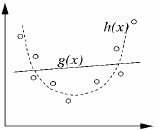
\includegraphics[width=.35\textwidth]{figs/underfitting}
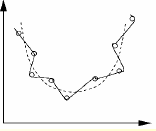
\includegraphics[width=.35\textwidth]{figs/overfitting}

Too simple vs. Too complex
\end{center}

\end{frame}

%%%%%%%%%%%%%%%%%%%%%%%%%%%%%%%%%%%%%%%%%%%%%%%%%%%%%%%%%%%%%%%%%%%%

\begin{frame}{Evaluation: Underfitting vs. Overfitting (cont.)}

Increasing the tree size, decreases the training and testing errors. However, at some point after (tree complexity), training error keeps decreasing but testing error increases

Many algorithms have parameters to determine the model complexity (e.g., in decision trees is the prunning parameter)

\begin{center}
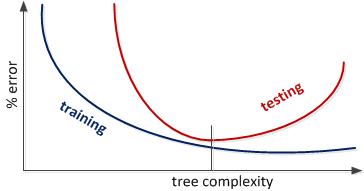
\includegraphics[width=.6\textwidth]{figs/overFittingDecisionTress}
\end{center}


\end{frame}


%%%%%%%%%%%%%%%%%%%%%%%%%%%%%%%%%%%%%%%%%%%%%%%%%%%%%%%%%%%%%%%%%%%%

% \begin{frame}{Evaluation: Costs}
% 
% Costs
% 
% 
% \end{frame}

%%%%%%%%%%%%%%%%%%%%%%%%%%%%%%%%%%%%%%%%%%%%%%%%%%%%%%%%%%%%%%%%%%%%

\subsection{Unsupervised Evaluation}

%%%%%%%%%%%%%%%%%%%%%%%%%%%%%%%%%%%%%%%%%%%%%%%%%%%%%%%%%%%%%%%%%%%%

\begin{frame}[fragile]{Unsupervised Evaluation}

\begin{itemize}
 \item \alert{Support}: the proportion of times that the rule applies
 \item \alert{Confidence}: the proportion of times that the rule is correct
\end{itemize}

\begin{verbatim}
if  colour = light and  #nuclei = 1 
Then #tails = 1   	
               (suport = 25%; 
                confidence = 50%)
}
\end{verbatim}


\end{frame}

%%%%%%%%%%%%%%%%%%%%%%%%%%%%%%%%%%%%%%%%%%%%%%%%%%%%%%%%%%%%%%%%%%%%%%%%%%%%%%%%
%%%%%%%%%%%%%%%%%%%%%%%%%%%%%%%%%%%%%%%%%%%%%%%%%%%%%%%%%%%%%%%%%%% Conclusions

%%%%%%%%%%%%%%%%%%%%%%%%%%%%%%%%%%%%%%%%%%%%%%%%%%%%%%%%%%%%%%%%%%
% \section{Conclusions and Future Work}
% %%%%%%%%%%%%%%%%%%%%%%%%%%%%%%%%%%%%%%%%%%%%%%%%%%%%%%%%%%%%%%%%
% 
% \subsection{Conclusions}
% 
% \begin{frame}{Conclusions and Future Work}
% 
% 
% 
% \end{frame}

%%%%%%%%%%%%%%%%%%%%%%%%%%%%%%%%%%%%%%%%%%%%%%%%%%%%%%%%%%%%%%%%%%%%%%%%%%%%%%%
% \begin{frame}{Conclusions and Future Work}
% 
% %\vskip0pt plus.5fill
% %\begin{block}{Conclusions}
% \begin{itemize}
%     \item FS obtains better accuracy than the datasets using all attributes
%     \begin{itemize}
%     \item
%       The wrapper model is superior to the filter model
%       \begin{itemize}
%         \item
%           It either improves the accuracy, or when the accuracy is not improved, 
% the models generated are much simpler, i.e., low no. of attributes; e.g., for 
% the JM1 dataset, the accuracy using IB1 wrapper is 72.01\% compared with 79.73\% 
% when using all attributes, however, it just needs less than 3 attributes for an 
% \emph{acceptable} accuracy.
%      \end{itemize}
%      \item The drawback is that the wrapper model is computationally expensive 
% (some runs took around a week to finish).
%    \end{itemize}
%    \item From the SE point of view, FS finds important attributes (for these 
% datasets, FS has removed most derived attributes.
% \end{itemize}
% %\end{block}
% 
% %\begin{block}{Future Work}
% \begin{itemize}
%         \item Future work: other datasets with more classes, how to deal and 
% analyze unbalanced datasets, etc.
% \end{itemize}
% %\end{block}
% 
% 
% \end{frame}




%%%%%%%%%%%%%%%%%%%%%%%%%%%%%%%%%%%%%%%%%%%%%%%%%%%%%%%%%%%%%%%%%%%%%%%%%%%%%%%

\section{References}

\begin{frame}{References}

\begin{scriptsize}

% \bibliographystyle{alpha}
\bibliographystyle{ieeetr}
% \bibliographystyle{unsrtnat} 
\bibliography{./references/references}
\end{scriptsize}


% \begin{thebibliography}{99}
% \bibitem{Boas} R. P. Boas,  Can we make mathematics intelligible?  
% \textit{Amer. Math. Monthly}, \textbf{88} (1981), 727--731.
% 
% \bibitem{Page} M. E. Page,  A Brief Citation Guide for Internet Sources in 
% History and the Humanities (Version 2.1),
% \begin{url}http://h-net.msu.edu/$\sim$africa/citation.html\end{url}.
% \end{thebibliography}

\end{frame}





\end{document}
